\begin{entry}{Q013}{Counting colourings with tensor networks}

\entrymeta{
  topic   = {Tensor networks; graph colouring; counting complexity.},
  est     = $\sim$30 minutes total --- longer than the usual daily entry.
    Part (a) alone is $\sim$12 minutes and is the core; (b) and (c) may be done
    in a second sitting.,
  origin  = {Sourced. The original exercise; the definitions of $e$ and $n$ from
    Section~1.5 are inlined so the statement stands alone.},
  source  = {J.~C. Bridgeman and C.~T. Chubb, \emph{Hand-waving and Interpretive Dance:
    An Introductory Course on Tensor Networks}, J.~Phys.~A \textbf{50}, 223001 (2017),
    \href{https://arxiv.org/abs/1603.03039}{arXiv:1603.03039}, Section~1.6,
    Problem~3.},
  prereq  = {Section 1.5 (computational complexity).},
  status  = open,
}

\begin{problem}
Recall the two binary tensors of Section~1.5. The tensor $e$ takes the value $1$ if and
only if all of its indices are equal, and $0$ otherwise; the tensor $n$ takes the value
$1$ if and only if all of its indices differ, and $0$ otherwise. Given an arbitrary
graph, build a tensor network by placing an $e$ tensor at each vertex and an $n$ tensor
in the middle of each edge, inheriting the connectivity of the graph, as in
Eq.~(1.19).

\begin{figure}[H]\centering
    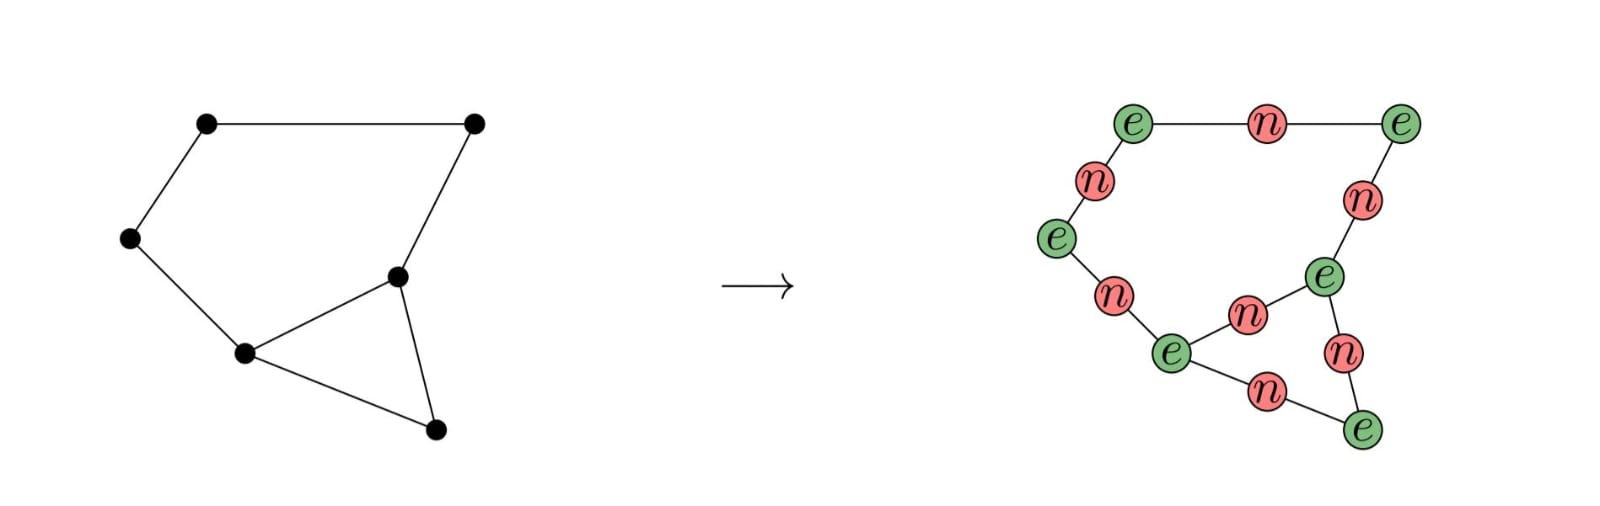
\includegraphics[width=0.7\linewidth]{images/tensorq3-1.jpeg}%
    \caption{The graph of Eq.~(1.19) and the tensor network built from it.}%
\end{figure}%

With $q$-dimensional indices, the nonzero contributions to this network are exactly the
vertex $q$-colourings of the graph, so its contraction counts them.

\begin{enumerate}[label=\textbf{(\alph*)},leftmargin=*]
  \item Calculate the contraction of the network of Eq.~(1.19) for bond dimension $q$,
        i.e.\ the number of three-colourings of the corresponding graph.
  \item Using the $e$ and $n$ tensors, construct a tensor network whose contraction gives
        the number of \emph{edge} colourings. For a planar graph, construct an analogous
        network counting \emph{face} colourings.
\end{enumerate}


\end{problem}

% ============================================================== solutions ===

\begin{solution}[Part (a)]
The equivalent tensor of e connected to two n, is
\begin{equation}
\begin{split}
    x_{a,b} &= \sum_{i,j}n_{a,i}e_{i,j}n_{j,b}\\
    &= \sum_{i,j} (1-\delta_{a,i})\delta_{i,j}(1-\delta_{j,b})\\
    &= \sum_{i} (1-\delta_{a,i})(1-\delta_{i,b})\\
    &= \delta_{a,b} + (q-2)
\end{split} 
\end{equation}

% requires \usepackage{tikz}
\usetikzlibrary{fit}
% requires \usetikzlibrary{fit}
\begin{figure}[H]\centering
\resizebox{\linewidth}{!}{%
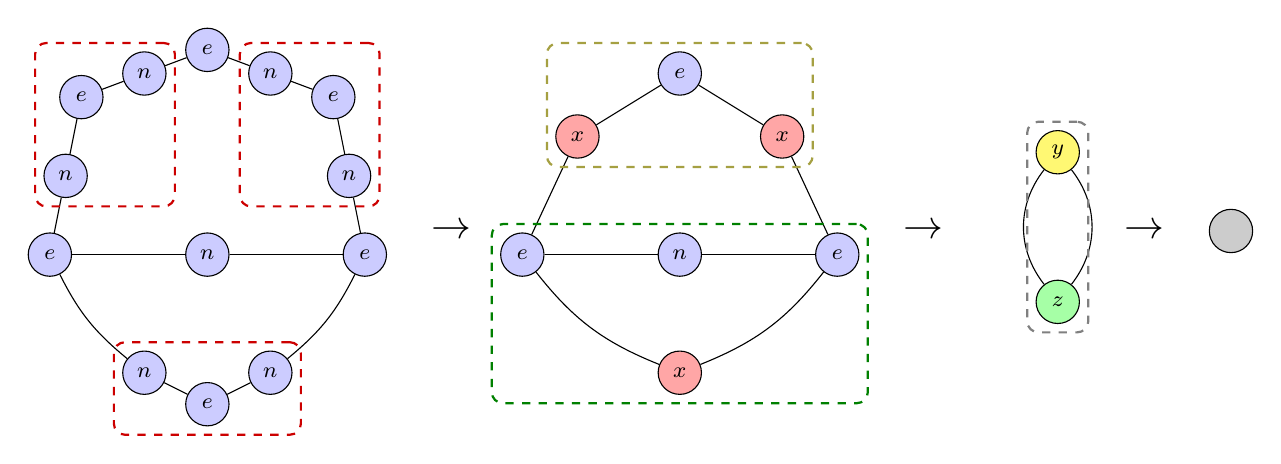
\begin{tikzpicture}[
  every node/.style={font=\footnotesize},
  ten/.style={circle,draw,minimum size=5.5mm,inner sep=0pt},
  blu/.style={ten,fill=blue!20},
  red/.style={ten,fill=red!35},
  yel/.style={ten,fill=yellow!55},
  grn/.style={ten,fill=green!35},
  cut/.style={draw,dashed,thick,rounded corners,inner sep=3pt},
]

%=================== PANEL 1 : original, relaid out ===================
\begin{scope}[shift={(0,0)}]
  % upper branch: v5 - v3 - v1 - v2 - v4
  \node[blu] (v1) at (2.0, 2.6) {$e$};
  \node[blu] (nb) at (1.2, 2.3) {$n$};
  \node[blu] (v3) at (0.4, 2.0) {$e$};
  \node[blu] (nc) at (0.2, 1.0) {$n$};
  \node[blu] (na) at (2.8, 2.3) {$n$};
  \node[blu] (v2) at (3.6, 2.0) {$e$};
  \node[blu] (nd) at (3.8, 1.0) {$n$};
  % axis
  \node[blu] (v5) at (0.0, 0.0) {$e$};
  \node[blu] (nn) at (2.0, 0.0) {$n$};
  \node[blu] (v4) at (4.0, 0.0) {$e$};
  % lower branch: v5 - v6 - v4
  \node[blu] (nf) at (1.2,-1.5) {$n$};
  \node[blu] (v6) at (2.0,-1.9) {$e$};
  \node[blu] (ng) at (2.8,-1.5) {$n$};

  \draw (v5)--(nc)--(v3)--(nb)--(v1)--(na)--(v2)--(nd)--(v4);
  \draw (v5)--(nn)--(v4);
  \draw (v5) to[bend right=12] (nf);
  \draw (nf)--(v6)--(ng);
  \draw (ng) to[bend right=12] (v4);

  \node[cut,red!80!black,fit=(nc)(v3)(nb)] {};
  \node[cut,red!80!black,fit=(na)(v2)(nd)] {};
  \node[cut,red!80!black,fit=(nf)(v6)(ng)] {};
\end{scope}

\node at (5.1,0.3) {\Large$\to$};

%=================== PANEL 2 : after x-reduction ===================
\begin{scope}[shift={(6.0,0)}]
  \node[blu] (w1) at (2.0, 2.3) {$e$};
  \node[red] (x2) at (0.7, 1.5) {$x$};
  \node[red] (x1) at (3.3, 1.5) {$x$};
  \node[blu] (w5) at (0.0, 0.0) {$e$};
  \node[blu] (nn) at (2.0, 0.0) {$n$};
  \node[blu] (w4) at (4.0, 0.0) {$e$};
  \node[red] (x3) at (2.0,-1.5) {$x$};

  \draw (w5)--(x2)--(w1)--(x1)--(w4);
  \draw (w5)--(nn)--(w4);
  \draw (w5) to[bend right=15] (x3);
  \draw (x3) to[bend right=15] (w4);

  \node[cut,yellow!60!black,fit=(x2)(w1)(x1)] {};
  \node[cut,green!50!black,fit=(w5)(nn)(x3)(w4)] {};
\end{scope}

\node at (11.1,0.3) {\Large$\to$};

%=================== PANEL 3 : y over z ===================
\begin{scope}[shift={(11.9,0)}]
  \node[yel] (y) at (0.9, 1.3) {$y$};
  \node[grn] (z) at (0.9,-0.6) {$z$};
  \draw (y) to[bend left=38]  (z);
  \draw (y) to[bend right=38] (z);
  \node[cut,gray,fit=(y)(z)] {};
\end{scope}

\node at (13.9,0.3) {\Large$\to$};

%=================== PANEL 4 : scalar ===================
\begin{scope}[shift={(14.5,0)}]
  \node[ten,fill=gray!40] at (0.5,0.3) {};
\end{scope}

\end{tikzpicture}}
\caption{Contraction of the network of Eq.~(1.19), redrawn so that the three
$n$--$e$--$n$ chains occupy disjoint regions. Red contours mark the chains replaced by
$x$; the yellow contour is $x$--$e$--$x\to y$; the green contour is the pair of vertices
joined by the parallel $n$ and $x$ bonds, $\to z$. Contracting $y$ against $z$ across the
double bond leaves a scalar.}
\end{figure}%

The upper part inside the yellow dashed line is equivalent to 
\begin{equation}
\begin{split}
    y_{a,b}&= \sum_{i,j}x_{a,i}e_{i,j}x_{j,b}\\
    &=\sum_{i,j} x_{a,i}\delta_{i,j}x_{j,b}\\
    &= \sum_{i} x_{a,i}x_{i,b}\\
    &= \sum_i (q-2)^2 + (q-2)(\delta_{a,i}+\delta_{i,b}) + \delta_{a,i}\delta_{i,b}\\
    &= q(q-2)^2+ 2(q-2) + \delta_{a,b}
\end{split}
\end{equation}
whereas for the below part inside the green dashed line is equivalent to 

\begin{equation}
\begin{split}
    z_{a,b}&= \sum_{i,j,k,l}e_{a,i,j}x_{j,l}n_{i,k}e_{k,l,b}\\
    &=\sum_{i,j,k,l}\delta_{a,i,j}x_{j,l}n_{i,k}\delta_{k,l,b}\\
    &= x_{a,b}n_{a,b}
\end{split}
\end{equation}
so
\begin{equation}
\begin{split}
    T&=\sum_{a,b} z_{a,b}y_{a,b}\\
    &= \sum_{a,b} (q(q-2)^2+ 2(q-2) + \delta_{a,b})((q-2)+\delta_{a,b})(1-\delta_{a,b})\\
    &= q(q-1)(q-2)^2[q^2-2q+2]
\end{split}
\end{equation}


\end{solution}

\begin{solution}[Part (b)]
These tensor $e$ and $n$ allows one to generalize the q-colouring counting problem by simple using $e$ in place of the counting object and $n$ used as the "adjacency mediator"  forcing that no adjacent objects have the same colour. To count the number of edges colouring you may draw a tensor network with $e$ in the edges and $n$ in the vertices, meanwhile to count the number of face colouring you draw a network with $e$ in the face( inside each polygon) and $n$ in the commom edges of the polygons. 
\end{solution}





\attempt{
  date        = ,
  time        = ,
  difficulty  = ,
  how it went = ,
}

\end{entry}